\section*{Physique (13 woints)}
\section*{Exercice 1 (3 points) : Propagation des ondes mécaniques et lumineuses}
Les phénomènes liés à la propagation des ondes mécaniques et lumineuses permettent de fournir des informations sur les milieux de propagation, et de déterminer certains paramètres caractéristiques. Cet exercice vise l'étude de quelques propriétés des ondes ultrasonores et des ondes lumineuses.

\section*{1. Propagation des ondes ultrasonores}
On considère un dispositif émetteur $E$ - récepteur $R$ d'ondes ultrasonores situé à la distance $d=17 c m$ d'un obstacle. Les ondes ultrasonores se propagent à partir de $E$ et se réfléchissent sur l'obstacle puis sont reçues par $R$ (Figure 1).

\begin{figure}[h]
\begin{center}
  \includegraphics[alt={},max width=\textwidth]{53bec4bf-ae8a-49fa-b6a9-4c685324fa09-3_177_565_989_1402}
\captionsetup{labelformat=empty}
\caption{Figure 1}
\end{center}
\end{figure}

1.1. Recopier sur votre copie, le numéro de la question, et écrire la lettre correspondante à la seule proposition vraie :

\begin{center}
\begin{tabular}{|l|l|}
\hline
A & Les ondes ultrasonores se propagent à la vitesse $c=3.10^{8} \mathrm{~m} . \mathrm{s}^{-1}$ \\
\hline
B & Le domaine de fréquences des ondes ultrasonores est compris entre 20 Hz et 20 kHz \\
\hline
C & Les ondes ultrasonores sont des ondes transversales \\
\hline
D & Les ondes ultrasonores sont des ondes mécaniques qui se propagent dans un milieu matériel élastique \\
\hline
\end{tabular}
\end{center}

1.2. La figure (2) donne l'oscillogramme de l'onde émise (a) et l'onde reçue (b).\\
Déterminer graphiquement la valeur du retard temporel $\tau$ entre les ondes (a) et (b).\\
1.3. Calculer la célérité des ondes ultrasonores dans l'air.\\
1.4. Recopier sur votre copie, le numéro de la question, et écrire la lettre correspondante à la seule proposition vraie.\\
L'élangalion d'un point $M$ du milieu de propagation, situé au

\begin{figure}[h]
\begin{center}
  \includegraphics[alt={},max width=\textwidth]{53bec4bf-ae8a-49fa-b6a9-4c685324fa09-3_430_652_1647_1311}
\captionsetup{labelformat=empty}
\caption{Figure 2}
\end{center}
\end{figure}

\begin{center}
\begin{tabular}{|l|l|l|l|}
\hline
$\mathbf{A}$ & $y_{M}(t)=y_{E}\left(t-1.10^{-3}\right)$ & $\mathbf{B}$ & $y_{M}(t)=y_{E}\left(t-5.10^{-4}\right)$ \\
\hline
$\mathbf{C}$ & $y_{M}(t)=y_{E}\left(t-2,5.10^{-4}\right)$ & $\mathbf{D}$ & $y_{M}(t)=y_{E}\left(t-5.10^{-3}\right)$ \\
\hline
\end{tabular}
\end{center}

\section*{2. Propagation des ondes lumineuses}
On éclaire une fente verticale de largeur $a$, à l'aide d'un laser qui donne une lumière monochromatique de longueur d'onde $\lambda$ et de fréquence $v$. On observe sur un écran placé à la distance $D$ de la fente, des taches lumineuses alternées. La largeur de la tache centrale est notée $L$.

\section*{Données :}
\begin{itemize}
  \item $D=1 \mathrm{~m} \quad ; \quad v=5.10^{14} \mathrm{~Hz} \quad ; \quad L=12 \mathrm{~mm}$
  \item Célérité de la lumière dans le vide (ou l'air) : $\mathrm{c}=3.10^{8} \mathrm{~m} . \mathrm{s}^{-1}$\\
2.1. Nommer le phénomène observé. Quel aspect de la lumière est mis en évidence ?\\
2.2. Recopier sur votre copie, le numéro de la question, et écrire la lettre correspondante à la seule proposition vraie.\\
L'expression de la largeur $a$ de la fente et sa valeur sont :
\end{itemize}

\begin{center}
\begin{tabular}{|l|l|l|l|}
\hline
$\mathbf{A}$ & $a=\frac{2 . c . L}{v . D} ; a=0,10 \mathrm{~mm}$ & $\mathbf{C}$ & $a=\frac{2 c . D}{v . L} ; a=0,10 \mathrm{~mm}$ \\
\hline
$\mathbf{B}$ & $a=\frac{c . D}{2 v . L} ; a=0,05 \mathrm{~mm}$ & $\mathbf{D}$ & $a=\frac{c . L}{2 v . D} ; a=0,12 \mathrm{~mm}$ \\
\hline
\end{tabular}
\end{center}

\section*{Exercice 2 (5 points) : Dinole RL - Circuit RLC série}
Le dipôle $R L$ et le circuit $R L C$ série montrent des comportements variés : $R L$ s'oppose aux variations du courant électrique, tandis que $\boldsymbol{R} \boldsymbol{L} \boldsymbol{C}$ série peut être siège d'oscillations électriques. L'étude de ces circuits peut se faire électriquement ou énergétiquement.\\
Cet exercice vise :

\begin{itemize}
  \item l'étude de la réponse d'un dipôle $\boldsymbol{R} \boldsymbol{L}$ à un échelon de tension ascendant;
  \item l'étude énergétique d'un circuit $R L C$ série.
\end{itemize}

\section*{Partie 1: Réponse d'un dipôle $R L$ à un échelon de tension ascendant}
Le circuit de la figure 1 comporte les éléments suivants :

\begin{itemize}
  \item un générateur idéal de tension de force électromotrice $E=4 V$;
  \item une bobine d'inductance $L$ et de résistance $r$;
  \item un conducteur ohmique de résistance $R=30 \Omega$;
  \item un interrupteur $K$.
\end{itemize}

À $t_{0}=0$, on ferme l'interrupteur, il s'établi un courant électrique avec un retard. La figure 2 donne l'évolution de la tension $u_{R}(t)$ aux bornes du conducteur ohmique.

\begin{center}
\begin{tabular}{|l|l|}
\hline
\includegraphics[max width=\textwidth, alt={}]{53bec4bf-ae8a-49fa-b6a9-4c685324fa09-4_323_362_1895_490}
 & \includegraphics[max width=\textwidth, alt={}]{53bec4bf-ae8a-49fa-b6a9-4c685324fa09-4_388_545_1867_1178}
 \\
\hline
Figure 1 & Figure 2 \\
\hline
\end{tabular}
\end{center}

\begin{enumerate}
  \item Indiquer l'élément qui est à l'origine du retard de l'établissement du courant dans le circuit.
  \item Établir l'équation différentielle vérifiée par l'intensité $i(t)$ du courant électrique lors de son établissement.
  \item Déterminer la valeur de l'intensité $I_{P}$ du courant dans le circuit en régime permanant.
  \item Calculer la valeur de $r$.
  \item Déterminer graphiquement la valeur de la constante de temps $\tau$ du circuit.
  \item Vérifier que $L=1,2 H$.
\end{enumerate}

\section*{Partie 2: Étude énergétique d'un circuit $R L C$ série}
On branche la bobine ( $L, r$ ) précédente en série avec un condensateur de capacité $C$ initialement chargé, et un conducteur ohmique de résistance $R^{\prime}$ (Figure 3).\\
La figure 4 donne l'évolution de la tension $u_{C}(t)$ aux bornes du condensateur.\\
\includegraphics[max width=\textwidth, alt={}, center]{53bec4bf-ae8a-49fa-b6a9-4c685324fa09-5_483_1659_589_212}

\begin{enumerate}
  \item Recopier sur votre copie le schéma du circuit et indiquer comment brancher un oscilloscope pour visualiser $u_{c}(t)$.
  \item Nommer le régime d'oscillations observé et l'expliquer du point de vue énergétique.
  \item Déterminer graphiquement la valeur de la pseudo période $T$ des oscillations.
  \item En considérant que la pseudo période $T$ est égale à la période propre $T_{0}$ des oscillations électriques sinusoïdales, calculer la valeur de $C$ (On prend $\pi^{2}=10$ ).
  \item Déterminer la valeur de la variation de l'énergie totale $\Delta \mathscr{E}$ du circuit entre les instants $t_{0}=0$ et $t_{1}=4 . T$.
\end{enumerate}

\section*{Exercice 3 (Spoints) : Etude dynamique et énergétique d'un systeme mécanique}
Le jeu du chariot impacteur pour enfant est une activité ludique qui consiste à lancer un chariot sur un rail rectiligne et incliné par rapport à l'horizontal. Le défi est réalisé lorsque le chariot percute une cible située à l'extrémité du rail.\\
Cet exercice vise :

\begin{itemize}
  \item l'étude dynamique du mouvement d'un solide sur un plan incliné ;
  \item l'étude énergétique d'un système \{solide-ressort\}.
\end{itemize}

\begin{enumerate}
    \item \begin{enumerate}
  \item On modélise le dispositif du jeu par un solide ( $S$ ) de centre d'inertie $G$ et de masse $m$ se déplaçant sur un rail rectiligne $A B$ de longueur $L$ incliné d'un angle $\alpha$ par rapport à l'horizontal (Figure 1). À l'instant $t_{0}=0$, le solide $(S)$ est lancé avec une vitesse initiale $\vec{V}_{0}$ de la position
\end{enumerate}

\begin{figure}[h]
\begin{center}
  \includegraphics[alt={},max width=\textwidth]{53bec4bf-ae8a-49fa-b6a9-4c685324fa09-5_341_533_1631_1361}
\captionsetup{labelformat=empty}
\caption{Figure 1}
\end{center}
\end{figure}

$A$.\\
On étudie le mouvement de ( $S$ ) dans un repère ( $O, \vec{i}, \vec{j}$ ) lié à la Terre supposé galiléen.\\
L'abscisse de $G$ à $t_{0}=0$ est $x_{G}=x_{0}=0$.\\
Données : $m=1 \mathrm{~kg} ; \alpha=25^{\circ} ; g=10 \mathrm{~m} . \mathrm{s}^{-2} ; L=A B=3 \mathrm{~m}$\\
Au cours de son mouvement, le solide subit des frottements équivalents à une force $\bar{f}$ constante colinéaire au vecteur vitesse et de sens opposé.\\
1.1. En appliquant la deuxième loi de Newton, montrer que l'expression de l'accélération $a_{G}$ de $G$ s'écrit : $a_{G}=-\left(g \cdot \sin \alpha+\frac{f}{m}\right)$.\\
1.2. La figure 2 donne le diagramme de vitesse de $G$.

\begin{figure}[h]
\begin{center}
  \includegraphics[alt={},max width=\textwidth]{53bec4bf-ae8a-49fa-b6a9-4c685324fa09-5_538_543_2051_1356}
\captionsetup{labelformat=empty}
\caption{Figure 2}
\end{center}
\end{figure}

1.2.1. Écrire l'expression numérique de l'équation de la vitesse de $G$.\\
1.2.2. Calculer l'intensité $f$ de la force de frottement.\\
1.2.3. Déterminer l'instant $t_{1}$ où le sens de mouvement de $(S)$ change.\\
1.2.4. Calculer la distance $d_{1}$ parcourue par le solide durant la phase de montée.\\
1.2.5. Déterminer la vitesse minimale $v_{0, \text { min }}$ avec laquelle le solide $(S)$ doit être lancé pour réaliser le défi.\\


    \item On réalise l'oscillateur \{solide $\mathrm{(S)}$, ressort\} en fixant le solide
$\mathrm{(S)}$ précédent à l'extrémité d'un ressort horizontal à spires non
jointives, de masse négligeable et de raideur $K$.

On écarte $\mathrm{(S)}$ de sa position d'équilibre d'une distance $X_{m}$, et
on le libère sans vitesse initiale à l'instant $t_{0}=0$. Le solide
$\mathrm{(S)}$ est animé d'un mouvement de translation rectiligne sinusoïdal
d'équation horaire ${x(t)=\num{5.e-2}\cdot\cos(2\pi\cdot t)~(\unit{\m})}$.

\vspace{3mm}
\begin{minipage}{0.60\linewidth}
    \begin{enumerate}
        \item Déterminer la valeur de $X_{m}$ et celle de la période propre $T_{0}$
              des oscillations.
        \item Calculer la valeur de la raideur $K$ (On prend $\pi^{2}=10$).
        \item On choisit l'état où le ressort n'est pas déformé comme état de
              référence de l'énergie potentielle élastique $E_{pe}$, et le plan
              horizontal contenant $G$ comme état de référence de l'énergie
              potentielle de pesanteur $E_{pp}$.
    
              La figure 3 donne les variations de l'énergie cinétique $E_{C}$ du
              solide $\mathrm{(S)}$ en fonction de l'élongation $x$ de $G$.
              \begin{enumerate}
                  \item Justifier que l'énergie mécanique du système se conserve.
                  \item Déterminer la valeur de l'énergie potentielle élastique
                        $E_{pe}$ lorsque $G$ atteint l'élongation maximale.
                  \item Calculer le travail $W(\vec{F})$ de la force exercée par le
                        ressort sur le solide $\mathrm{(S)}$, lorsque $G$ passe de
                        la position d'élongation $x=X_{m}$ à la position
                        d'élongation $x_{0}=0$.
              \end{enumerate}
    \end{enumerate}
\end{minipage}
\hfill
\begin{minipage}{0.38\linewidth}
    \begin{figure}[H]
        \centering
        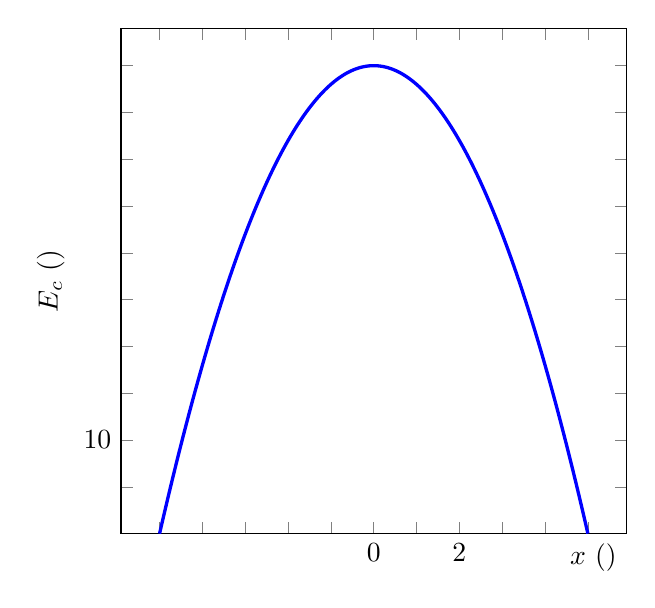
\begin{tikzpicture}
            \def\K{40}
            \def\Xm{0.05}
            \begin{axis}[
                    xmin=-0.059,xmax=0.059,
                    ymin=0,ymax=54,
                    width=8cm,height=8cm,
                    xlabel=$x~(\unit{\cm})$,
                    ylabel=$E_{c}~(\unit{\mJ})$,
                    every axis x label/.append style={
                        at={(1,0)},anchor=north east,
                    },
                    scaled ticks=false,
                    xtick distance=0.01, ytick distance=5,
                    xticklabels={,,,,,,0,,2}, yticklabels={,,,10},
                    minor tick num=0,
                ]
                \addplot[domain=-\Xm:\Xm,samples=200,
                    very thick,blue] {0.5*\K*(\Xm^2-x^2)*1e3};
            \end{axis}
        \end{tikzpicture}
        \caption{}
        \label{fig:2bac_svt_national_2025_rattrapage_phys_ex3_3}
    \end{figure}
\end{minipage}




\end{enumerate}


